\section{三种方法的产出形态对比}
\label{sec:forms}

三种方法最本质的差别并不只在数值精度，而在\textbf{产出形态}：一维杆只给出一条轴向曲线，Q4 给出连续二维场，CST 给出分块常应力场。表~\ref{tab:forms} 从未知量、应力表示、主要产出和后处理能力四个维度归纳这一差异；图~\ref{fig:forms} 用同一 S1 工况、同一 $40\times8$ 网格并排展示三种产出。

\begin{table}[htbp]
  \centering
  \caption{三种方法的产出形态对比。表中的“信息量”指对截面内应力分布与端部局部变形的描述能力，而非数值精度。}
  \label{tab:forms}
  \footnotesize
  \begin{tabular}{@{}p{0.17\textwidth}p{0.25\textwidth}p{0.25\textwidth}p{0.25\textwidth}@{}}
\toprule
维度 & 一维杆单元 & Q4 等参元 & CST 三角形 \\
\midrule
每节点自由度 & 1（$u_x$） & 2（$u_x,u_y$） & 2（$u_x,u_y$） \\
单元未知量 & 2 & 8 & 6 \\
单元刚度 & $2\times2$，闭式 & $8\times8$，$2\times2$ 高斯积分 & $6\times6$，显式 \\
应力表示 & 单元常数（按平衡恢复） & 单元内双线性 & 单元常数（常应变） \\
主要产出 & $u(x)$、$\sigma(x)$ 两条一维曲线 & 连续 $\sigma_x$ 云图、任意点应力 & 分块 $\sigma_x$ 云图、节点恢复场 \\
信息量/代价 & 信息最少、自由度最省 & 场连续、代价中等 & 单元数约为 Q4 两倍，局部应力不连续 \\
后处理 & 截面平均、1D 判据 & 高斯点应力、梯度保真、剪切能比 & 面积加权恢复、对角线离散 \\
典型适用 & 杆系快速估算、A/B 级工况 & 光滑二维场、端部复核 & 复杂几何、快速原型 \\
\bottomrule
\end{tabular}

\end{table}

\begin{figure}[htbp]
  \centering
  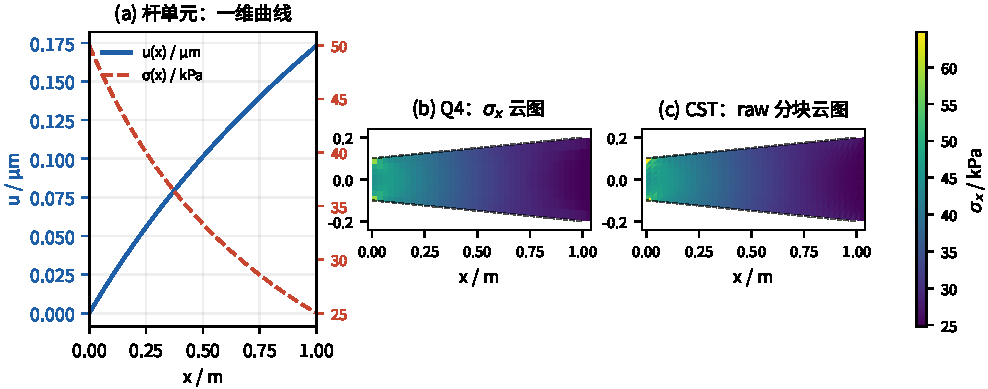
\includegraphics[width=\textwidth]{figures/fig_production_forms.pdf}
  \caption{同一 S1 工况（$40\times8$）下三种方法的产出形态。现象：杆单元只产生 $u(x)$、$\sigma(x)$ 两条一维曲线；Q4 云图在单元内与跨单元均连续；CST raw 云图呈明显分块，块界即单元边界。解读：曲线形式自由度最省、信息量最低，适合一维杆系快速估算；Q4 的双线性插值与高斯点应力给出连续场，适合光滑应力场与端部复核；CST 的常应变假设导致分块，需面积加权节点恢复或更密网格才能得到平滑场，这也是后文单独量化对角线离散度的原因。}
  \label{fig:forms}
\end{figure}

产出形态差异带来三点直接后果。第一，评价指标必须与产出形态匹配：杆单元应比较截面平均位移/应力与一维判据，Q4/CST 则应比较二维点值或全场误差；若只用端部位移，会掩盖 CST 局部应力的分块误差。第二，CST 的“raw 云图”不能直接作为应力结果使用，面积加权节点恢复或更密网格是必要的后处理；本文因此同时报告 raw 与 recovered 两套剖面。第三，若工程只关心轴力与截面平均应力，一维杆的曲线已足够；若关心端部应力集中、楔形边缘的横向应力或局部屈服，则必须使用 Q4 或更密 CST。图~\ref{fig:forms}(b) 与 (c) 的视觉差异，正是第~\ref{sec:results} 节精度差异的直观来源。
